\appendix 
%\appendixpage
\chapter{OSI Model}
\label{osi}
  \begin{center}
  \begin{tabular}{|lc|}
  \hline
  7: &
  Application Layer \\
  & (e.g. DNS, DHCP) \\
  \hline
  6: &
  Presentation Layer \\
  & (e.g. telnet) \\ 
  \hline
  5: &
  Session Layer \\
  & (e.g. RPC) \\
  \hline
  4: &
  Transport Layer \\
  & (e.g. TCP, UDP) \\
  \hline
  3: &
  Network Layer \\
  & (e.g. IPv4, IPv6) \\
  \hline  
  2: &
  Data Link Layer \\
  & (e.g. MAC) \\ 
  \hline  
  1: &
  Physical Layer \\
  & (e.g. Ethernet, Wi-Fi) \\
  \hline
\end{tabular}
\end{center}

The seven layer OSI model is a logical grouping of the types of protocols found
in computer networks. Each layer is dependent only on the layer directly below
it. 

The TCP/IP model is a similar, but simpler model of networking.

\chapter{Additional zClient-zServ Messages}
\label{zClient}
I extended the zClient-zServ protocol to expose some of the features,
previously only available through the vtysh, to the routing protocol
implementations. 

\begin{center}
	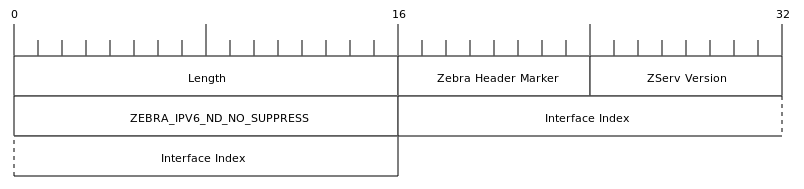
\includegraphics[width=0.9\linewidth]{../Diagrams/Packets/nd_no_suppress.png}
\end{center}

The first of these messages is one to enable sending Router Advertisements. It
works by stopping NDP messages from being suppressed. There is also a
corresponding message to turn these RAs off again. 

\begin{center}
	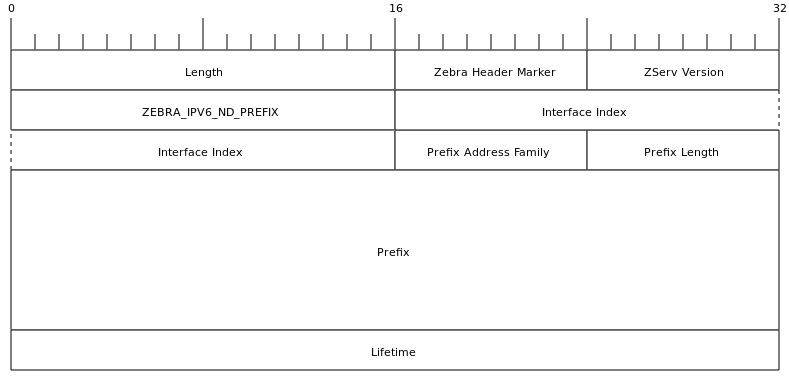
\includegraphics[width=0.9\linewidth]{../Diagrams/Packets/ipv6_nd_prefix.png}
\end{center}

The next message adds a prefix prefix to the RAs. This is used to advertise a
new assigned prefix. There is also a similar messages to remove the prefix.


\begin{center}
	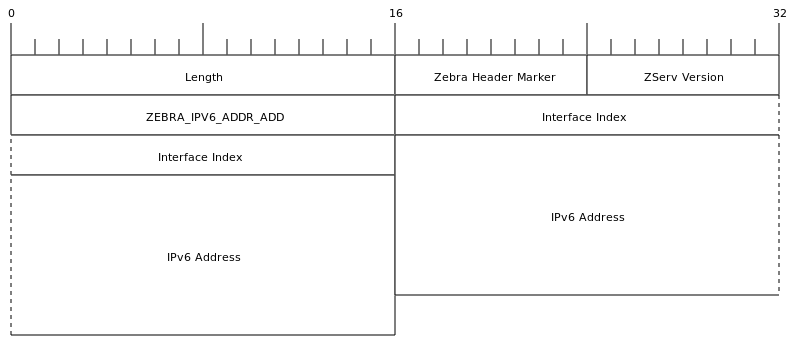
\includegraphics[width=0.9\linewidth]{../Diagrams/Packets/addr_add.png}
\end{center}

The final message adds an IPv6 Address to a specified interface. In my
implementation this was used to associate a prefix an interface for the routing
table calculations. Again, there is also a message to remove the address.

\chapter{Netkit}
\begin{center}
	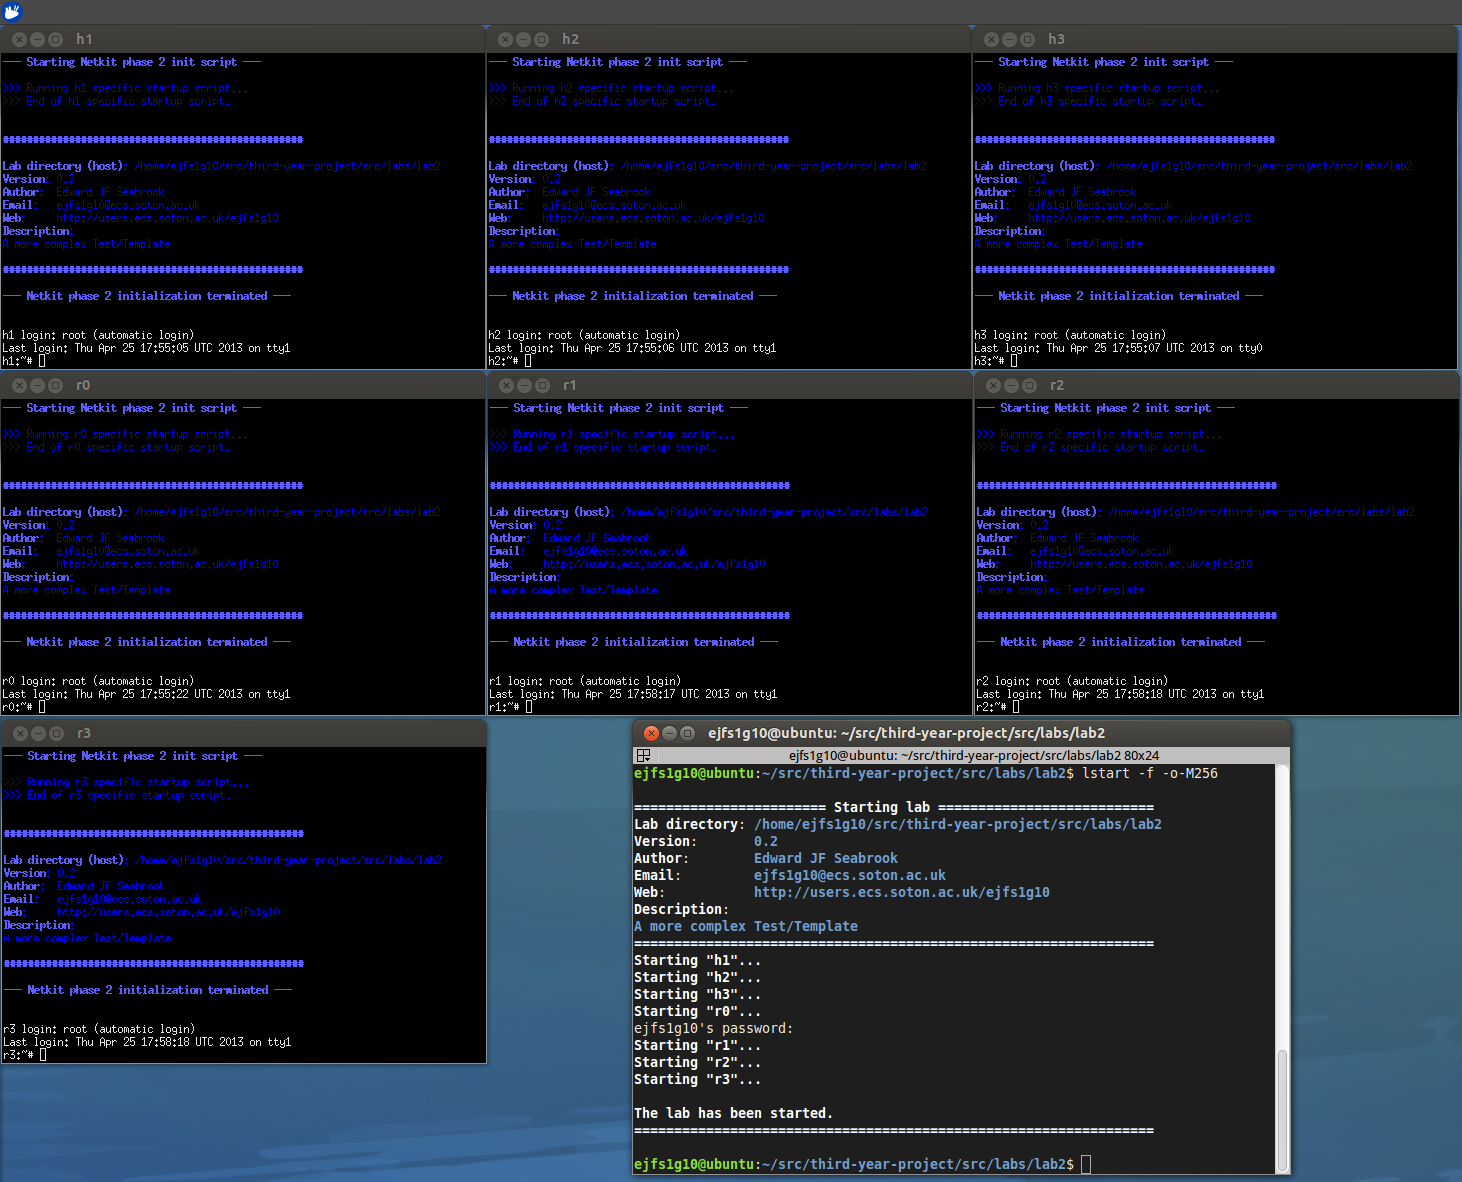
\includegraphics[width=\linewidth]{../Diagrams/Netkit/NetkitScreenshot.png}
\end{center}

Above is a screen shot of a typical Netkit session.  

Netkit instances are started with \texttt{vstart \$NAME}.

A lab is a collection of VMs and collision domains, described in a
configuration file. Labs are started with \texttt{lstart}. It is often useful
to allocate the VMs in the lab more memory using the flag \texttt{-o-M}n, where
n is the size of the memory to allocate in megabytes.

\chapter{radvdump}
\label{radvdump}
This \texttt{radvdump} output shows the contents of the router advertisements
made by one of my quagga instances. The prefix fc35:6225:4b8:6::/64 is a ULA
that was generated automatically.

\lstinputlisting{../Issues/radvdump.md}

\chapter{Github Stats}
\label{GithubStats}
GitHub offers various graphics that can be used to visualise the progress and
patterned in the project. 

\section{Github Commit Graph}
\begin{center}
	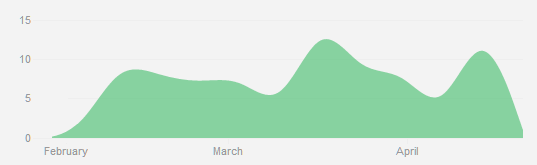
\includegraphics[width=\linewidth]{../Diagrams/Stats/GitHubCommitGraph.png}
\end{center}

This commit graph shows all of the commits that I made to my fork of Quagga.
The graph shows that I began working on my implementation in early February and
worked steadily, peaking at the beginning of the Easter vacation. The second
peak is when I began working on testing.

\section{Github Punchcard}
\begin{center}
	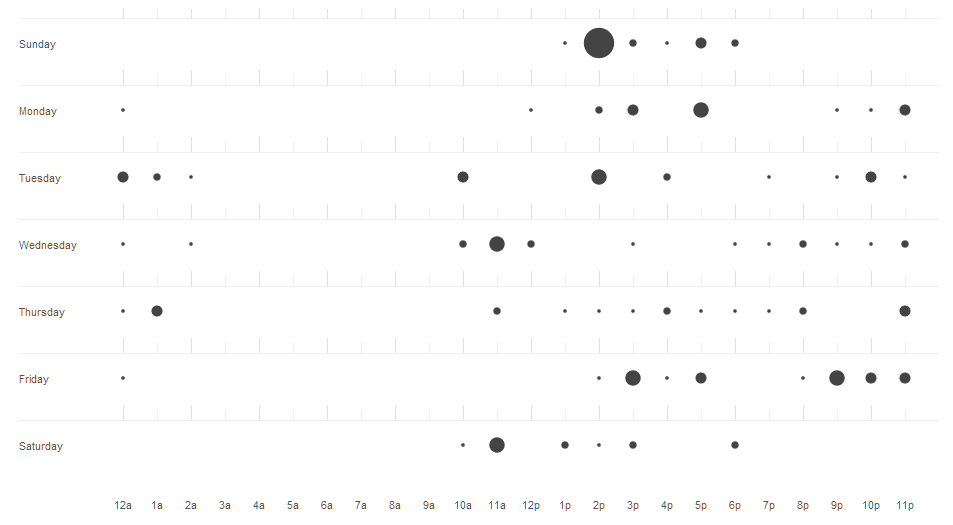
\includegraphics[width=\linewidth]{../Diagrams/Stats/GitHubPunchCard.png}
\end{center}

This punch card shows the time of day, and day of the week that I made 
my contributions. The graph is for my documentation repository as the code
repository contained many commits by other authors.

\chapter{Alix2d3}
As the project progressed it became clear that they Alix2d3s were not as useful
as was originaly believed, thanks to discovery of the briliant software package
Netkit. I did however undertake testing on the Alix2d3s. If someone wished to
repeat my experimentation, the following guides would be helpful. 

\section{Ubuntu Installation Guide}

 This guide\cite{germanGuide} offered a comprehensive list of steps that need to
 be taken to install Ubuntu Linux on a PC Engines alix2d3\cite{alix2d3}.  The article is
 written in German but using Google translate I was able to follow it as it is
 mainly a list of shell commands.

 The process begins with installing the compact flash card as a device on an
 existing Ubuntu desktop PC\@. Next the card is partitioned using \texttt{fdisk},
 the card is then formatted as ext2 (a Linux file system type) using
 \texttt{mk2fs}. The card is then mounted in the file system, using
 \texttt{mount} and a small installation of Linux is copied to the card using
 \texttt{debootstrap} to provide a base system.

 Several settings and devices are linked to the flash cards mount point and
 \texttt{chroot} is used to simulate booting into the new install. The required
 configuration files are edited (e.g.\@ network interface settings) and essential
 software packages (such as \texttt{Vim}, \texttt{SSH}, \texttt{sudo}, and
 \texttt{APT}) are installed. A boot loader such as \texttt{GRUB} is also
 installed and configured.

 Next, the flash card is safely removed, and  inserted into the alix2d3. The
 alix2d3 is then powered on. Using a USB to Null Model cable connecting a PC to
 the alix2d3's serial port, a terminal connection can be established using {\bf
 cu}. I had a few problems using this device (\texttt{ttyUSB0}) but I was able to
 fix this problem using \texttt{chown}. This terminal connection can be used to
 aid the boot process and ensure that there are no Magic ELF errors. Once the
 alix2d3 is up and running it is possible to disconnect the serial cable and
 access it over \texttt{SSH} alone.

 \section{Quagga Installation Guide}

 \subsection{Normal Installation}
This procedure turned out to be far more difficult that anticipated.

First, ensure all the dependencies are present. The easiest
way I have found to do this is to use:

\texttt{sudo apt-get build-dep quagga}

This should fetch all the packages that Quagga depends on. These do not need to
be built from source, since I do not modify them. libtool and libreadline need
to be installed separately. 


Next it should be possible to run \texttt{\@./bootstrap}, this creates the
configure script; run it:

\begin{quote}
\texttt{sudo \@./configure \\ --sysconfdir=/usr/local/quagga \\ --localstatedir=/usr/local/quagga}
\end{quote}

The configure script will prompt you to create a user called quagga. Do this by:

\begin{quote}
\texttt{sudo adduser quagga}

\texttt{sudo mkdir /usr/local/quagga}

\texttt{sudo chown quagga:quagga /usr/local/quagga}
\end{quote}

It is now time to run \texttt{make}. See Appendix~\ref{cross_compile} for more
information about this. I had issues with making zebra, I fixed them by
manually editing the Makefile in \texttt{\@./zebra}, adding \texttt{-lcap} to
\texttt{LIBS}\@. This issue no longer occurs with the latest release of quagga.

Next run \texttt{sudo make install}. This should install everything -- the daemons
should have installed themselves to \texttt{/usr/local/sbin}.

Finally a little bit of configuration is required. \texttt{cd
/usr/local/quagga} Either make a real config file for the daemons (zebra and
ospf6d), or just create file containing ``password test''.

You should now be able to run ospf6d. If you can't, try \texttt{ldconfig}.

\subsection{Cross Compilation}
\label{cross_compile}
Since Alix2d3s are very slow, building Quagga can be incredibly slow. The make
parts alone can take around 15 minutes. (XORP had an even slower compile time,
in the order of hours) 

To overcome this issue it is possible to compile the source code on a much
faster machine (e.g.\@ desktop pc) and copy it across. 

Since modern machines use a 64bit architecture rather than 32bit like the
Alix2d3s, the compiler must be set up correctly. The cflag \texttt{-m32
-march=i386} can be used. This can be done by appending
\texttt{--with-clfags=`-m32 -march=i386i'} to \texttt{\@./configure}.

I initially had problems with this compilation. I resolved the issues by going
back to basics and trying to compile a simple helloworld program for the Alix.
Turns out I was missing \texttt{gcc-multilib}. This can be installed with \texttt{apt}.

\chapter{vtysh}
\label{vtysh}
Commands are added using the macro DEFUN and the function install.

I added the commands:
\begin{itemize}
	\item \texttt{show ipv6 ospf6 prefix aggregated} \\
		Used to display all aggregated prefixes in the system.
	\item \texttt{show ipv6 ospf6 prefix allocated} \\ 
		Used to display the only aggregated prefixes that were allocated to this
		router only.
	\item \texttt{show ipv6 ospf6 prefix assigned X} \\
		Used to display the prefixes that have been assigned to a given interface
		by the prefix assignment algorithm. 


	\item \texttt{enable $\rightarrow$ configure terminal 
		$\rightarrow$ ipv6 allocate-prefix X:X::X:X/M} \\
		Used to manually allocate a new aggregated prefix to the routers.
	\item \texttt{enable $\rightarrow$ configure terminal
		$\rightarrow$ no ipv6 allocate-prefix X:X::X:X/M} \\
		Used to remove a previously allocated aggregated prefix.
\end{itemize}

\chapter{Test Results}
\label{testResults}
Of the twenty testcases that I produced, all of them now pass. The following is an
example of the output of my unit testing code: 

\begin{lstlisting}
Testcase 5  %{\color{green} OK}%
Toal interface count: 2 
 Aggregated Prefix: fc00::/48
 Aggregated Prefix: fc00:1::/48
Total Aggregated Prefix count: 2 
 eth0's Assigned Prefix count: 2
  Assigned Prefix: fc00:0:0:1::/64
   Not Valid
   Deprecation Thread
  Assigned Prefix: fc00:0:0:3::/64
 eth1's Assigned Prefix count: 2
  Assigned Prefix: fc00:0:0:2::/64
  Assigned Prefix: fc00:1::/64
   Pending Thread
Total Assigned Prefix count: 4 
\end{lstlisting}
